\documentclass[12pt,letterpaper]{article}
\usepackage{natbib}

%Packages
\usepackage{pdflscape}
\usepackage{fixltx2e}
\usepackage{textcomp}
\usepackage{fullpage}
\usepackage{float}
\usepackage{latexsym}
\usepackage{url}
\usepackage{epsfig}
\usepackage{graphicx}
\usepackage{amssymb}
\usepackage{amsmath}
\usepackage{mathtools}
\usepackage{bm}
\usepackage{array}
\usepackage[version=3]{mhchem}
\usepackage{ifthen}
\usepackage{caption}
\usepackage{hyperref}
\usepackage{amsthm}
\usepackage{amstext}
\usepackage{enumerate}
\usepackage[osf]{mathpazo}
\usepackage{dcolumn}
\usepackage{lineno}
\usepackage{dcolumn}
\usepackage{mathtools}

\DeclarePairedDelimiter\abs{\lvert}{\rvert}%
\DeclarePairedDelimiter\norm{\lVert}{\rVert}%
\newcolumntype{d}[1]{D{.}{.}{#1}}

\pagenumbering{arabic}


%Pagination style and stuff
\linespread{2}
\raggedright
\setlength{\parindent}{0.5in}
\setcounter{secnumdepth}{0} 
\renewcommand{\section}[1]{%
\bigskip
\begin{center}
\begin{Large}
\normalfont\scshape #1
\medskip
\end{Large}
\end{center}}
\renewcommand{\subsection}[1]{%
\bigskip
\begin{center}
\begin{large}
\normalfont\itshape #1
\end{large}
\end{center}}
\renewcommand{\subsubsection}[1]{%
\vspace{2ex}
\noindent
\textit{#1.}---}
\renewcommand{\tableofcontents}{}
%\bibpunct{(}{)}{;}{a}{}{,}

%---------------------------------------------
%
%       START
%
%---------------------------------------------

\begin{document}

%Running head
\begin{flushright}
Version dated: \today
\end{flushright}
\bigskip
\noindent RH: Characters correlation

\bigskip
\medskip
\begin{center}

\noindent{\Large \bf Effect of discrete character correlation on tree inference}
\bigskip

\noindent {\normalsize \sc Thomas Guillerme$^1$$^*$, and Martin D. Brazeau$^1$}\\
\noindent {\small \it 
$^1$Imperial College London, Silwood Park Campus, Department of Life Sciences, Buckhurst Road, Ascot SL5 7PY, United Kingdom.\\}
\end{center}
\medskip
\noindent{*\bf Corresponding author.} \textit{guillert@tcd.ie}\\ 
\vspace{1in}

%Line numbering
\modulolinenumbers[1]
\linenumbers

%---------------------------------------------
%
%       ABSTRACT
%
%---------------------------------------------

\newpage
\begin{abstract}
blablabla
\end{abstract}

\noindent (Keywords: )\\

\vspace{1.5in}

\newpage 


%---------------------------------------------
% LaTeX tips for modifying/editing the document:
%---------------------------------------------
% - You can comment using the percentage sign. I suggest you use the % sign alone for commenting out sections of the text:
%       e.g. "This is a really long sentence %because this sentence is very long." Here the % is used for ignoring the end of the sentence (but for some reason you want to keep track of it).%
%       For comments as in verbose comments, I suggest you use "%MB:":
%       e.g. "This is a really long sentence %because this sentence is very long. %MB: yeah, no shit!" 
% - For optimal version control, write only one sentence per line (for more precise track changes)
% - To build the pdf, use command+B in Sublime.
% - Because of the bibliography, the pdf needs to be build in the same folder that contains "References.bib" and "sysbio.bst"
% - For citing papers, you must put their bibtex reference in the "References.bib" file and then you can use the following sysbio tags:
%        \cite{bibtexBob2000} for citing within a sentence: "Bob (2000)"
%        \citep{bibtexBob2000} for citing within brackets: "(Bob, 2000)"
%        \citep[Before:][-After]{bibtexBob2000} for citing within brackets with additional text: "(Before: Bob, 2000 -After)"
%        \citealt{bibtexBob2000} for citing without brackets: "Bob, 2000"
%        You can put more cites in each \cite tag by separating them with commas.
% - For equation, find every details here: https://en.wikibooks.org/wiki/LaTeX/Mathematics
% - For titles and stuff, the hierarchy goes \section{}, \subsection{}, \subsubsection{} and so forth...
% - For bullet points or enumerations you can use:
%       \begin{itemize}
%           \item my first bullet point/enumeration
%       \end{itemize}
%       With replacing "itemize" by "enumerate" for enumeration.




%---------------------------------------------
%
%       INTRODUCTION
%
%---------------------------------------------
\section{Introduction}

The last six years have seen a fantastic expansion of the use of discrete morphological data in macroevolutionary studies.
Traditionally confined to ``classic'' cladistic studies, these methods have recently been widely expanded and improved whether based on the models and methods for inferring phylogenies \citep[e.g.][]{heath2014fossilized,Wright01072016} or to combine them with molecular data \citep[e.g.][]{pyrondivergence2011,ronquista2012}.
In parallel, much development has also been done on pre-phylogenetic analysis \citep[e.g. data collection;][]{morphobank} as well as on post-phylogenetic analysis \citep[e.g. morphological disparity analysis;][]{Close2015,Claddis}.
Nonetheless, using discrete morphological data in macroevolutionary studies comes with several caveats based to the nature of data used \citep{Guillerme2016146,bapst2017combined}; the coding of this data \citep{Brazeau2011,simoes2017giant}; the inference method \citep{spencerefficacy2013,wrightbayesian2014,OReilly20160081,puttick2017uncertain,goloboff2017weighted} or the dating methods \citep{Arcila2015131,o2016tips}.

One aspect of the data, however, is often neglected: the correlation between morphological characters.
In fact, the assumption of character independence is at the base of phylogenetic inference and as been mentioned or implied throughout the history of phylogenetic methods \citep[e.g.][]{joysey1982problems,felsenstein1985phylogenies,lewisa2001,felsenstein2004inferring}.
Nowadays, this assumption of character independence is nearly always accepted as a fact and rarely tested or questioned in empirical datasets.
However - especially for discrete morphological data - this assumption of independence is probably violated more often than not due to the sheer nature of phylogenetic data.
In practice, dependence between characters can be induced in at least three different ways:

\begin{itemize}
    \item \textbf{Biological induce dependence between characters:} this is the result of a link between two characters through development and/or biological function.
    These links are readily understood through developmental biology or understanding of shared function between features \citep{goswami2006morphological,goswami2010,goswami2014macroevolutionary}.
    One trivial example would be the link between lower and upper molar characters in mammals: one character describing a feature of a lower molar will be expected to be correlated to another character describing another feature of the associated upper molar.

    \item \textbf{Evolutionary induced dependence between characters:} this is the result of sets of characters co-evolving along branches in the phylogeny.
    The character's correlation is thus due to shared evolutionary history of these characters.
    Many methods have been developed to study these correlations, especially since they can provide us with a lot of information on how specific groups acquired specific characteristics \citep{Lande1983,Maddison1990,Pagel1994,Pagel2006,Grabowski2016}.
    For example, the apparition of the jaw as a character in gnatosthomes correlates with a whole sweep of characters present in modern gnatosthomes (e.g. beaks, tribosphenic molars, jaw protrusion, etc.). %TG: this links to inapplicable data!

    \item \textbf{Coding induced dependence between characters:} this is the results of researchers methodology for defining or/and coding discrete morphological characters \citep{Brazeau2011,simoes2017giant}.
    These dependences could be due to methodological errors. 
    For example one could define a character describing a particular feature on a left molar as well as another character describing the same feature on a right molar.
    It is worth noting that these dependences could also be due to the nature of the available data, especially in palaeontology.
    For example, when only one fragmentary molar is available to describe a specimen, researchers have to ``extract'' as much phylogenetic information from the available data as possible, potentially inducing correlations.
\end{itemize}

\noindent Of course, the three sources of dependences can also be correlated to each other: characters describing the left and right lower/upper molars will have induced dependence due to the modularity of the molars, their shared history and the duplicated coding!

As mentioned above, these sources of dependence between characters are well studied in biology.
Biological and evolutionary dependences are inherent parts to evo-devo and maroevolution and best practices to avoid coding induced dependences are commonly known and applied.
However, eventually, all these characters, whether they are independent or not are analysed through phylogenetic inferences softwares that are blind to these distinctions.
This introduces a new, less studied, source of character dependence:

\noindent \textbf{Software induced correlation between characters:} this is the result how software actually interprets the differences between characters.
I.e. the vast majority of phylogenetic software ignores both the character's definition and the different states signification (simply treating them as different/similar tokens) leading to dependence between characters.
For example, in a matrix containing four cetartiodactyles - say a pig (e.g. \textit{Sus}), a deer (\textit{Cervus}), a hippo (\textit{Hippopotamus}) and a whale (\textit{Balaenoptera}) - and four characters - say (\textbf{C1}: presence (1) or absence (0) of an astragal; \textbf{C2}: presence (0) or absence (1) of baleens; \textbf{C3}: presence (0) or absence (1) of a left astragal with a double pulley; \textbf{C4}: presence (0) or absence (1) of a right astragal with a double pulley - resulting in the following matrix:

\begin{table}
\center
    \begin{tabular}{r|cccc}
            & C1 & C2 & C3 & C4\\
        \hline
        \textit{Sus} & 1 & 1 & 1 & 1\\
        \textit{Cervus} & 1 & 1 & 1 & 1\\
        \textit{Hippopotamus} & 1 & 1 & 1 & 1\\
        \textit{Balaenoptera} & 0 & 0 & 0 & 0\\
    \end{tabular}
    \caption{Example of a matrix with software induced character correlation. \textbf{C1}: presence (1) or absence (0) of an astragal; \textbf{C2}: presence (0) or absence (1) of baleens; \textbf{C3}: presence (0) or absence (1) of a left astragal with a double pulley; \textbf{C4}: presence (0) or absence (1) of a right astragal with a double pulley.}
    \label{Tab:example_matrix}
\end{table}

In the example in Table \ref{Tab:example_matrix}, the characters \textbf{C1} and \textbf{C2} are the most likely to be truly independent; characters \textbf{C3} and \textbf{C4} suffer from a a coding induced dependency; characters \textbf{C1} and \textbf{C3}/\textbf{C4} have an evolutionary induce dependency and again, characters \textbf{C2} and \textbf{C3}/\textbf{C4} are likely to be independent.
Yet a phylogenetic software will treat all these four characters in exactly the same way: only the sheer difference between the different character states tokens will be used in order to infer a phylogenetic tree.
It is thus still unclear what will be the effect of characters correlation on phylogenetic inference: how does these correlation really affect topology?

If the three induced sources of correlation are fairly well studied, their actual interpretation in phylogenetic inference, has, to our knowledge, never been studied through a simulation protocol.
In this study, we formally assess the effect of discrete character's correlation using simulated and empirical data.
We propose a new metric to measure the difference between characters (as a proxy for these three sources of correlation) and a protocol to modify discrete morphological matrices to increase/decrease the overall differences/similarities between characters.
We found that blabalbal


% However, only several attempts have been made on the actual effect of characters correlation on phylogenetic inference with two notable exceptions of \cite{Davalos01072014} on empirical data and \cite{ZouConvergence} on molecular data. %TG: put that somwhere


\section{Methods}

We applied the following simulation protocol to assess the effect of characters correlation (Fig.\ref{Fig:outline}):
\begin{enumerate}
    \item \textbf{Simulating matrices}: we simulated discrete morphological matrices with 25, 75 and 150 taxa for 100, 350 and 1000 characters, hereafter called the ``normal'' matrices.
    \item \textbf{Modifying matrices}: we modified the ``normal'' matrices by duplicating characters in order to maximise or minimise characters differences (hereafter called respectively ``maximised'' and ``minimised'' matrices) by removing respectively the least or most different characters and replacing them randomly by the remaining characters.
    We also randomly duplicated characters from the ``normal'' matrices without biasing towards maximising or minimising character difference to create randomised matrices (hereafter called the ``randomised'' matrices - equivalent to a null expectancy).
    \item \textbf{Inferring topologies}: we inferred the topologies from the ``normal'', ``maximised'', ``minimised'' and ``randomised'' matrices using both Maximum Parsimony and Bayesian inference (hereafter called the ``normal'', ``maximised'', ``minimised'' and ``randomised'' trees).
    \item \textbf{Comparing topologies}: finally, we compared to topologies in two ways: (1) first we compared the ``normal'' to the ``randomised'' trees to assess our simulation protocol; (2) second, we compared the ``maximised'' and ``minimised'' trees to the ``randomised'' and ``normal'' trees respectively to measure the effect of character correlation on topology.
\end{enumerate}
Each steps are described below in more details, as well as our proposed definition of the Character Difference metric.

\begin{figure}[!htbp]
\centering
   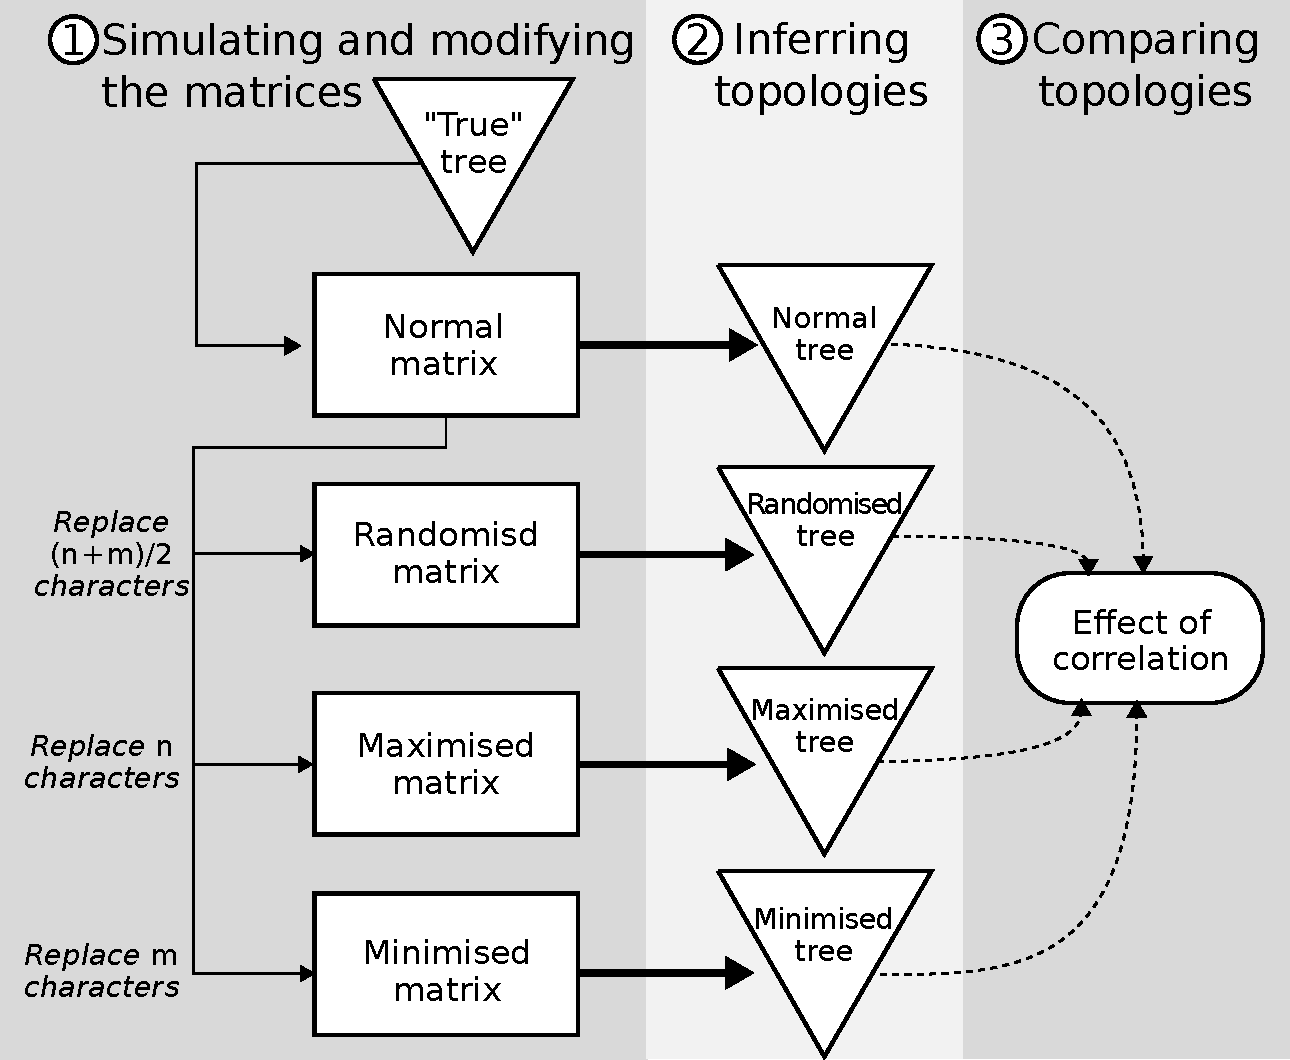
\includegraphics[width=0.9\textwidth]{Figures/outline.pdf}
\caption{Outline of the simulation protocol: the first step includes both the simulation and the modification of the matrices (thin solid lines); the second step includes tree inference using Maximum Parsimony and Bayesian inference (thick solid lines); the third step includes comparing the resulting tree topologies (dashed lines).}
\label{Fig:outline}
\end{figure}

\subsection{Measuring differences between characters}
We define characters as being correlated if they give the same phylogenetic information.
In order to measure this similitude in phylogenetic information, we propose a new distance metric to measure the difference between two characters:

\subsubsection{Characters Difference (CD)}
\begin{equation}
    CD_{(x,y)} = 1 - \left(\frac{\abs*{\frac{\sum_{i}^{n}\abs{x_{i} - y_{i}}}{n}-\frac{1}{2}}}{\frac{1}{2}}\right)
\end{equation}

\noindent Where $n$ is the number of taxa with comparable data and $x_i$ and $y_i$ are each characters states for the characters $x$ and $y$ and the taxa $i$.
$CD$ is a continuous distance metric valid in a mathematical sense (see Supplementary Material 1).
Since we are considering differences as being only Fitch-like (i.e. non-weighted and non-ordinate), we calculated the difference between character states in a qualitative way.
Two same character states tokens have a difference of $0$ and two different ones have a difference of $1$ (e.g. $0 - 0 = 0$ or $1 - 8 = 1$).
Additionally, we only consider differences for taxa with shared information \citep[i.e. a Gower distance;][]{GowerDist}.
In order to facilitate and standardise characters states comparison, we standardised each characters by arbitrarily modifying their character states tokens by order of appearance.
In other words, we replaced all the occurrences of the first token to be $1$, the second to be $2$, etc.
This way, a character \texttt{A = \{2,2,3,0,0,3\}} would be standardised as \texttt{A' = \{1,1,2,3,3,2\}} \citep[following the \textit{xyz} notation in][p.13]{felsenstein2004inferring}.
Note that in terms of phylogenetic signal, both \texttt{A} and \texttt{A'} are exactly identical (forming three distinct groups).

When the character difference is equal to $0$, it means that characters convey the same phylogenetic signal.
When the character difference is equal to $1$ it means it conveys the most different signal.
For example with three characters \texttt{A = \{0,1,1,1\}}, \texttt{B = \{1,0,0,0\}} and \texttt{C = \{0,1,2,3\}}, $CD_{(A,B)} = 0$ and $CD_{(A,C)} = 1$.

\subsection{Simulating discrete morphological matrices}
To simulate the matrices we applied a protocol very similar to \citep{Guillerme2016146}.
First, we generate random birth-death trees with the birth ($\lambda$) and death ($\mu$) parameters sampled from a uniform ($0$,$1$) distribution maintaining $\lambda$ $>$ $\mu$ using the diversitree \texttt{R} package \citep[v0.9-8;][]{fitzjohndiversitree2012} and saving the tree after reaching either 25, 75 or 150 taxa.
For each tree, we arbitrarily set the outgroup to be the first taxa (alphabetically) thus effectively rooting the trees on this taxa.
These trees are hereafter called the ``true'' trees.
We then simulated discrete morphological characters on the topology of these trees using the either of the two following models:
\begin{itemize}
    \item The morphological HKY-binary model \citep{OReilly20160081} which is an HKY model \citep{HKY85} with a random states frequency (sampled from a uniform distribution $(0,1)$ and scaled to sum to $1$) and using a transition/transvertion rate of $2$ \citep{douadycomparison2003} but where the purines (A,G) were changed into state $0$ and the pyrimidines (C,T) in state $1$.
    This model has the advantage of not favouring Bayesian inference \citep[since it doesn't use a M$k$ model;][; see below]{OReilly20160081} but the downside of it is it can only generate binary state characters \citep[or 4 states;][]{puttick2017uncertain}.
    \item To generate more than binary states characters, we used the M$k$ model \citep{lewisa2001}.
    We draw the number of character states with a probability of $0.85$ for binary characters and $0.15$ for three state characters \citep{Guillerme2016146}.
    This model assumes a equal transition rate between character states that might seem overly simplifying and excludes other observed transition patterns \citep[e.g. Dollo characters;][]{Dollo,wright2015came}.
    Recently however, \cite{Wright01072016} have shown that an equal rate transition is still the most present in empirical data.
\end{itemize}

\noindent For each character, both models (morphological HKY-binary or M$k$) where chosen randomly and ran with an overall evolutionary rate drawn from a gamma distribution ($\beta$ = $100$ and $\alpha$ = $5$).
This low evolutionary rate values allowed to reduce the number of homoplasic character changes and thus reinforce the phylogenetic information in the matrices.
We re-simulated every invariant characters to obtain a matrix with no invariant characters.
To ensure that our simulation where reflecting realistic observed parameters, we only selected matrices with Consistency Indices superior to $0.26$ \citep{OReilly20160081}.

It can be noted that this Consistency Index threshold might favor Maximum Parsimony inference (since we measured this index using quick parsimony trees) yet the evolutionary models of each character is slightly in favor of Bayesian inference (since, on average, half the characters evolved following a M$k$ model).

For each trees with 25, 75 or 150 taxa we generated matrices with 100, 350 and 1000 characters following \cite{OReilly20160081}.
The matrices where generated using the \texttt{dispRity R} package \citep{thomas_guillerme_2016_55646}.
To estimate the variance of our simulations and assess the effect of our random parameters, we repeated this step 40 times resulting in 360 ``normal'' morphological matrices.

\subsection{Modifying the matrices}
We calculated the pairwise Character Differences for each generated matrices using the \texttt{dispRity R} package \citep{thomas_guillerme_2016_55646}. %TG: TO IMPLEMENT! 
We then modified the matrices to either maximise or minimise the pairwise character differences for each matrices using three different algorithms.
For maximising the pairwise differences between characters, we selected the characters that where the most similar to all the others (i.e. with an average character difference $<$$0.25$) and replaced them randomly by any of the remaining characters.
This operation increased the overall pairwise character difference in the matrix thus making the characters more dissimilar.
Conversely, for minimising the pairwise character differences, we selected the most dissimilar characters (i.e. with an average character difference $<$$0.75$) and randomly replaced them with the remaining ones.
Finally, because this operation effectively changes the weight of characters (i.e. giving the characters $<$$0.25$ or $>$$0.75$ a weight of $0$ and giving the randomly selected remaining characters a weight of +$1$), we randomly replaced the average number of characters replaced in the character maximisation and minimisation by any other characters as a randomised expectation modification (i.e. randomly weighting characters).
This step resulted in a total of 1440 matrices (hereafter called the ``normal'', ``maximised'', ``minimised'' and ``randomised'' matrices - see Fig. \ref{Fig:modif_matrix} for an illustration).
The algorithms for the three modifications are available on GitHub@@@. %(Modifying_matrices.html) %TG: "@@@" is my "to replace" sign.

\begin{figure}[!htbp]
\centering
   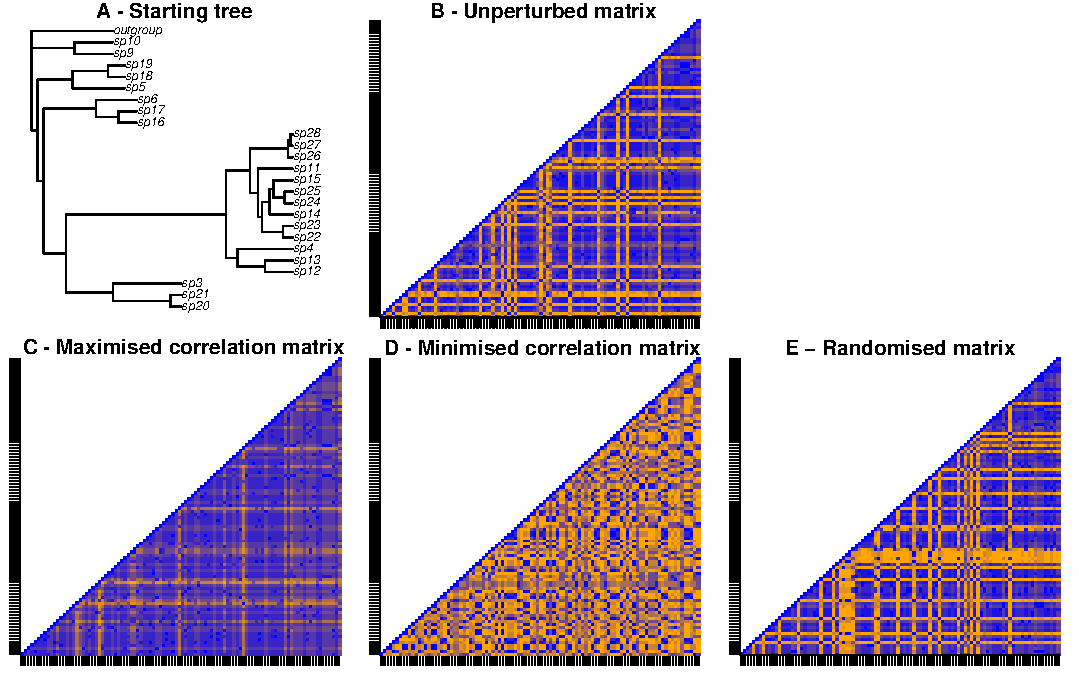
\includegraphics[width=1\textwidth]{Figures/Modif_matrix.pdf}
\caption{Example illustration of the protocol for modifying matrices. The matrices represent the pairwise character differences for 100 characters. Blue colours correspond to low character differences and orange colours correspond to high character differences. \textbf{A} - a random Birth-Death tree is simulated and used for generating the normal matrix (\textbf{B}), characters in this matrix are then removed or duplicated to favour maximised character difference (\textbf{C}), minimised it (\textbf{D}) or randomise it (\textbf{E}).}
\label{Fig:modif_matrix}
\end{figure}

\subsection{Inferring topologies}
We inferred the topologies in both Bayesian and Maximum Parsimony using MrBayes \citep[v3.2.6;][]{Ronquist2012mrbayes} and PAUP* \citep[v4.0a151;][]{swofford2001paup} respectively.
For both methods, we set the arbitrarily chosen outgroup as an outgroup in the models.
The Maximum Parsimony inference was run using a heuristic search with random sequence addition replicate 100 times with a limit of $5\times10^6$ rearrangements per replicates (\texttt{hsearch addseq=random nreps=100 rearrlimit=5000000 limitperrep=yes}).

The Bayesian inference was run using an M\textit{k} model with ascertainment bias and four discrete gamma rate categories (M\textit{kv} $4\Gamma$ - \texttt{lset nst=1 rates=gamma Ngammacat=4}) with an variable rate prior an exponential (0.5) shape (\texttt{prset ratepr=variable Shapepr=Exponential(0.5)}).
We ran two runs of 6 chains each (2 hot, 4 cold) for a maximum of $1\times10^9$ generations with a sampling every 200 generations.
We automatically stopped the MCMC when the average standard deviation of split frequencies (ASDSF) between both runs fell below 0.01 (with a diagnosis every $1\times10^4$ generations - \texttt{mcmc nruns=2 Nchains=6 ngen=1000000000 samplefreq=200 printfreq=2000 diagnfreq=10000 Stoprule=YES stopval=0.01 mcmcdiagn=YES}).
Due to cluster hardware requirements an to save some time, when chains didn't converged and the runs exceeded 5GB each, we aborted the MCMC and computed the consensus tree from the uncoverged chains.
In practice, these few MCMC got stuck at an ASDSF around (but not below) 0.01.

A strict majority rule tree was then calculated for both Bayesian an Maximum Parsimony trees.
For the Bayesian consensus trees, the 25\% first trees of the posterior tree distribution were excluded as a burnin.
The 2880 tree inferences took around 1 CPU century on the Imperial College High Performance Computing Service \citep[2-3GHz clock rate;][]{HPC}.

\subsection{Comparing topologies}
We compared the topologies using the same approach as in \cite{Guillerme2016146}: we measured both the Robinson-Fould distance \citep{RF1981} and the Triplets distance \citep{dobson1975triplets} between the trees inferred from the ``maximised'', ``minimised'' and ``randomised'' matrices and the tree inferred from the ``normal'' matrix.
We ran two types of comparisons, (1) the effect of Character Difference on recovering the ``normal'' topology by comparing the ``maximised'', ``minimised'' and ``randomised'' trees to the ``normal'' tree (Figs \ref{Fig:RF_results_best} and \ref{Fig:Tr_results_best}); and (2) the signal to noise ratio induced by the simulation protocol by comparing the ``randomised'' trees to the ``normal'', ``maximised'' and ``minimised'' trees (Figs \ref{Fig:RF_results_rand} and \ref{Fig:Tr_results_rand}). 

The metrics scores where obtained using the TreeCmp java script \citep{Bogdanowicz2012}.
The measurements where then standardised using the Normalised Tree Similarity metric \citep[i.e. centering the metrics scores using the mean metric score for 1000 pairwise comparisons between random trees with $n$ taxa;][]{Bogdanowicz2012,Guillerme2016146}.
When the normalised metric has a score of $1$ it means both trees are identical, when it has a score of $0$ it means the trees are no more different than expected by chance and when it has a score $<0$ the trees are more different than expected by chance.
The normalised score for both metrics thus reflects two distinct aspects of tree topology: (1) the Normalised Robinson-Fould Similarity reflects the conservation of clades (i.e. a score close to $1$ indicates that most clades are identical in both trees); and (2) the Normalised Triplets Similarity reflects the position of taxa (i.e. a score close to $1$ indicates that most taxa have the same neighbours in both trees).

\section{Results}

\begin{figure}[!htbp]
\centering
   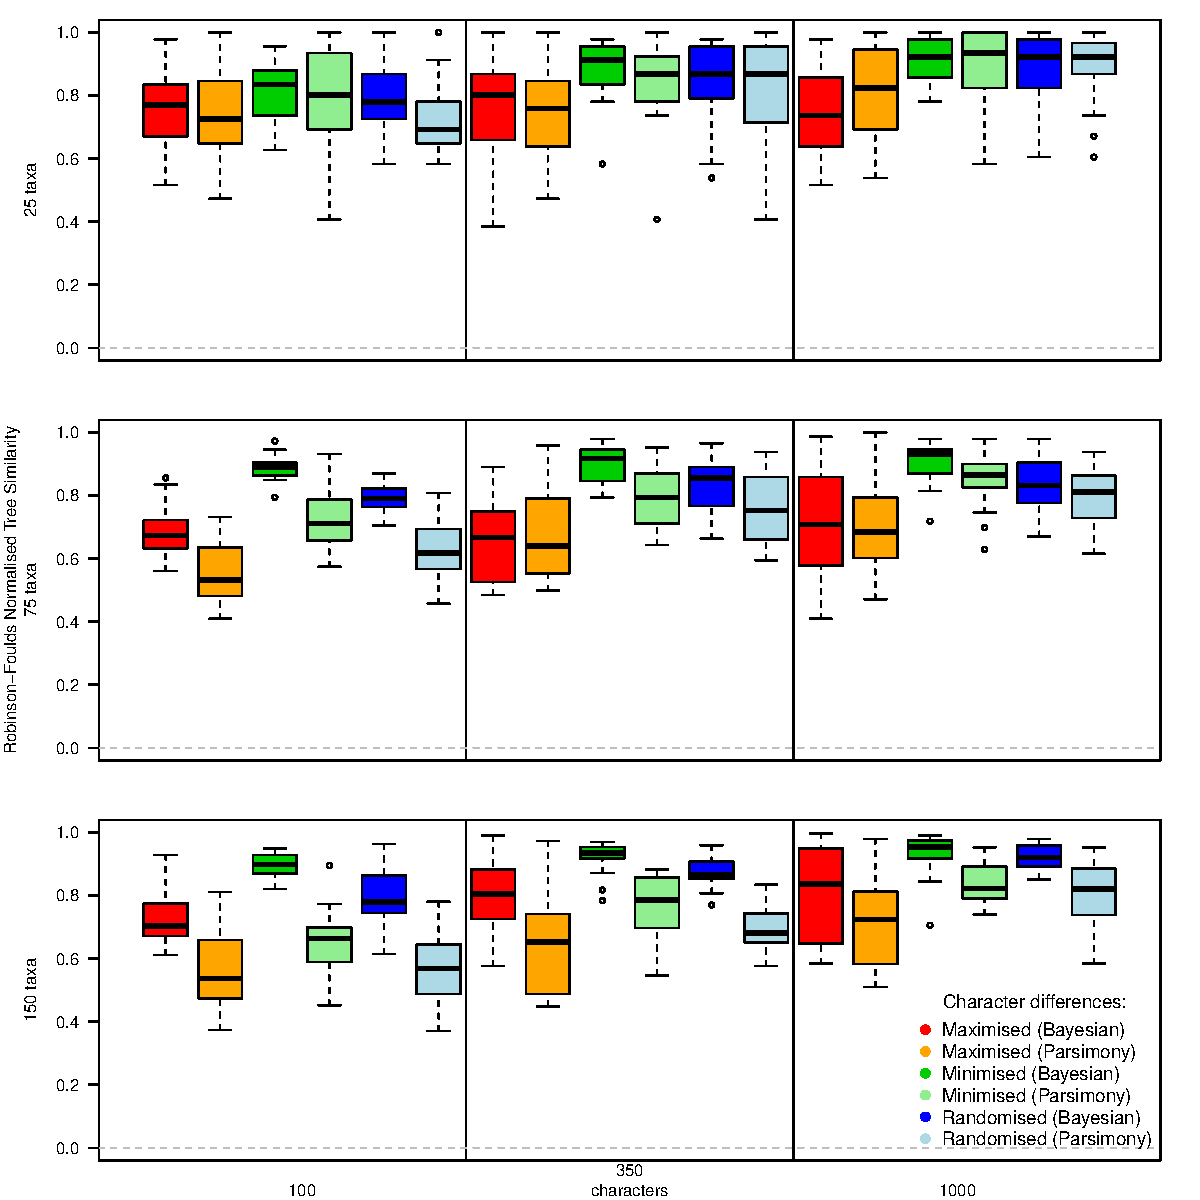
\includegraphics[width=1\textwidth]{Figures/RF_results_best.pdf} %TG: These figures will be cleaned up once I have the final results.
\caption{Effect of Character Difference on recovering the ``best'' topology. The y axis represents the Normalised Tree Similarity using Robinson-Fould distance for matrices with 25, 75 and 150 taxa from top to bottom respectively. The x axis represents the different Character Difference scenarios and tree inference method with the Maximised Character Difference in Bayesian (red) and under Maximum Parsimony (orange), the Minimised Character Difference in Bayesian (dark green) and under Maximum Parsimony (light green) and the Randomised Character Difference in Bayesian (dark blue) and under Maximum Parsimony (light blue) for matrices of 100, 350 and 1000 characters in the panels from left to right.}
\label{Fig:RF_results_best}
\end{figure}


\begin{figure}[!htbp]
\centering
   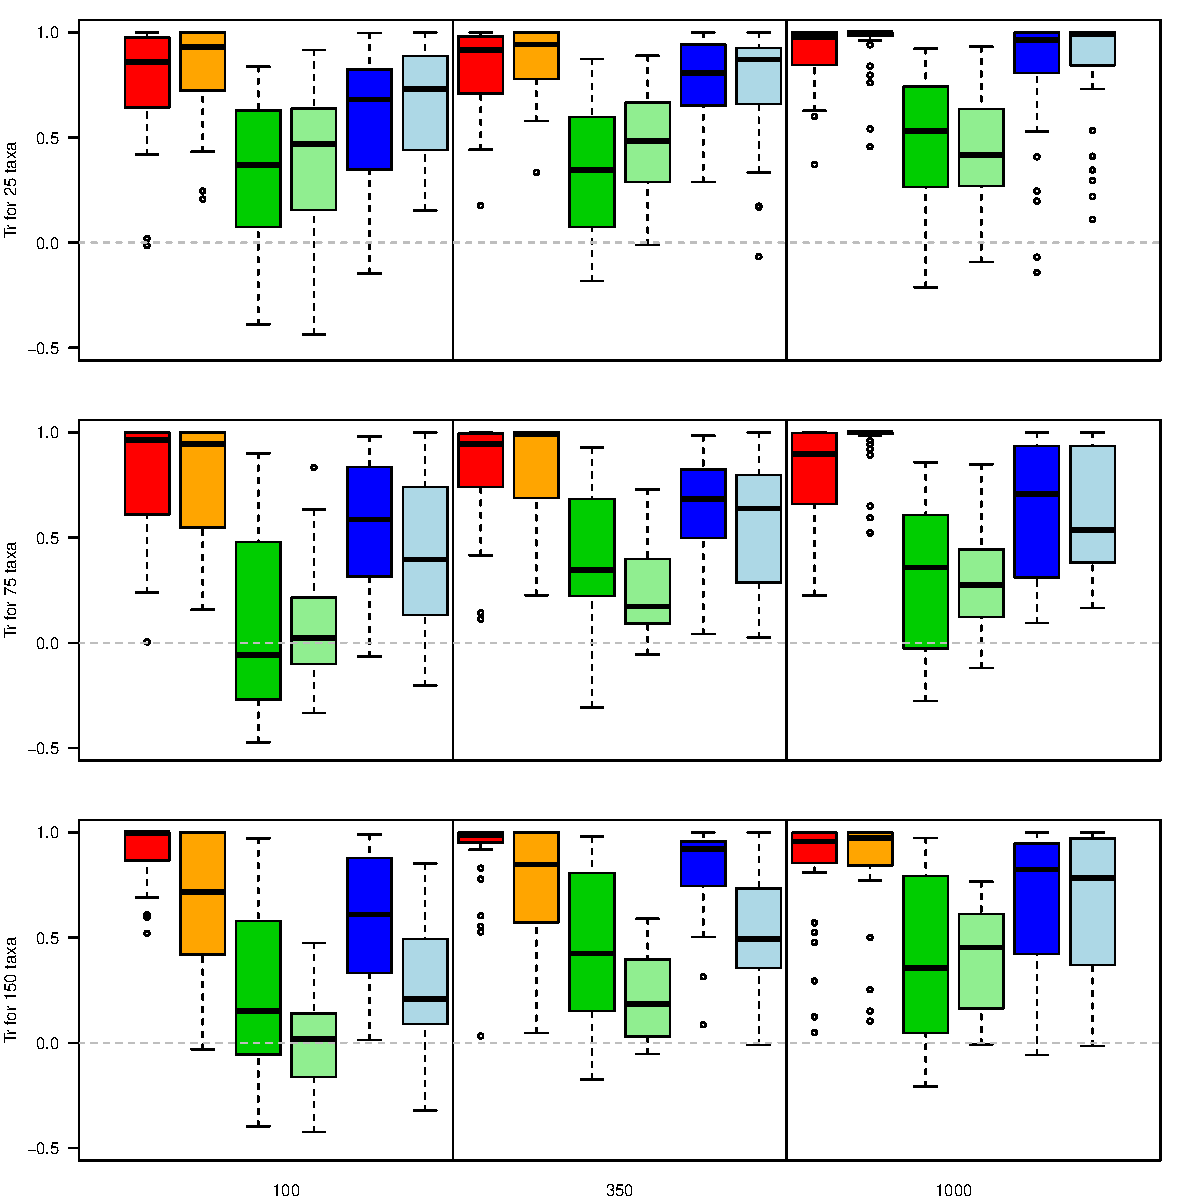
\includegraphics[width=1\textwidth]{Figures/Tr_results_best.pdf} %TG: These figures will be cleaned up once I have the final results.
\caption{Effect of Character Difference on recovering the ``best'' topology. The axis are identical to figure \ref{Fig:RF_results_best} but y axis represents the Normalised Tree Similarity using Triplets distance.}
\label{Fig:Tr_results_best}
\end{figure}


\begin{figure}[!htbp]
\centering
   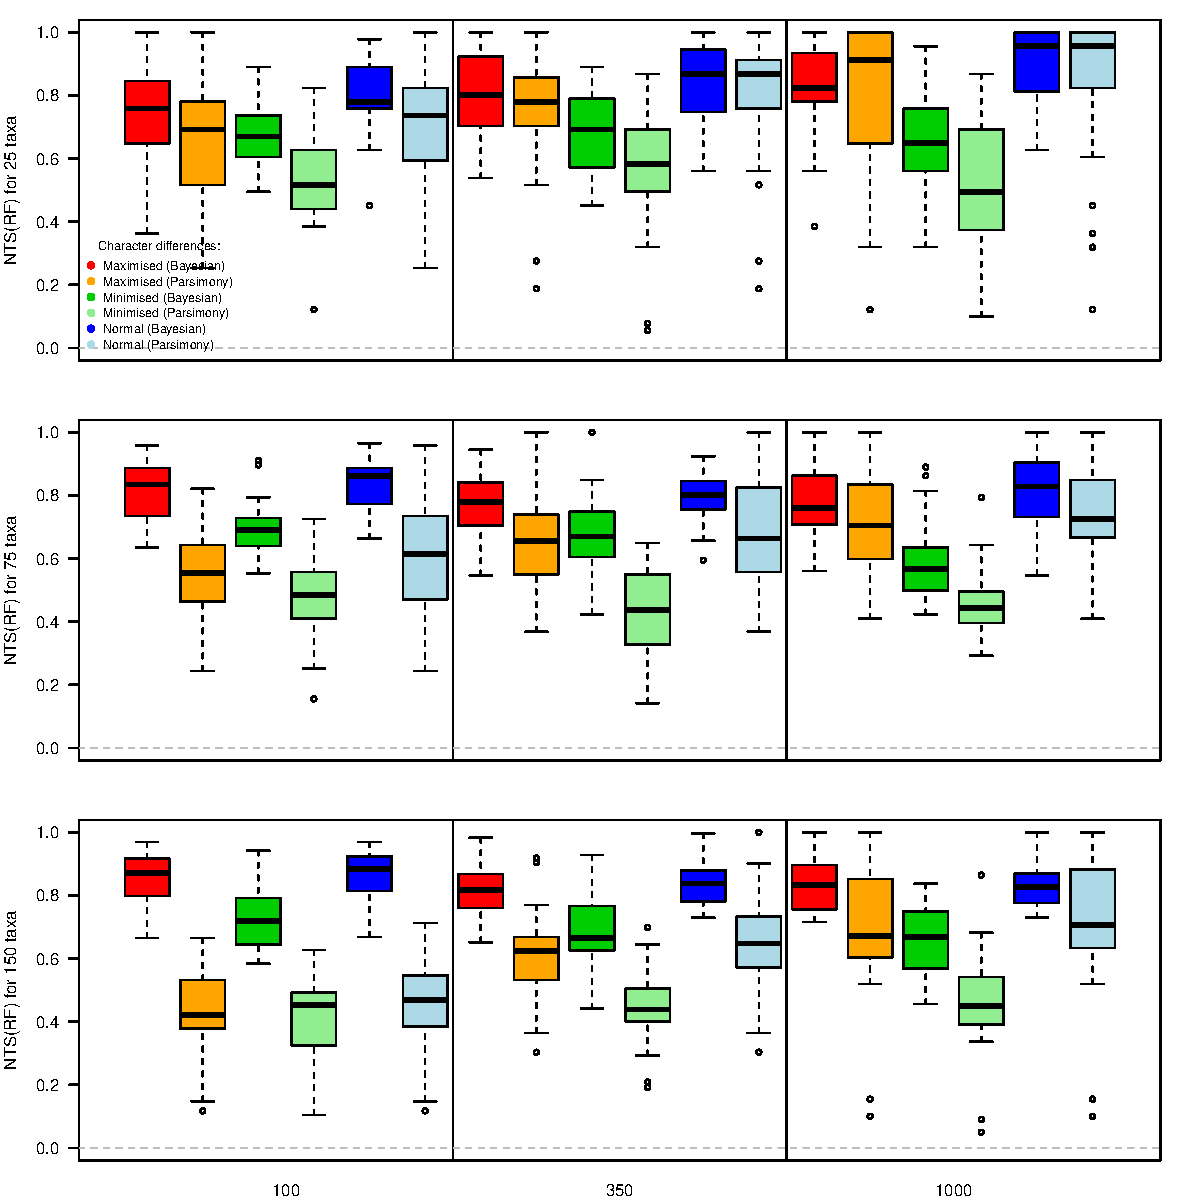
\includegraphics[width=1\textwidth]{Figures/RF_results_null.pdf} %TG: These figures will be cleaned up once I have the final results.
\caption{Effect of Character Difference on recovering the ``random'' topology. The axis are identical to figure \ref{Fig:RF_results_best} but y axis represents the Normalised Tree Similarity using Ronbinson-Fould distance.}
\label{Fig:RF_results_rand}
\end{figure}


\begin{figure}[!htbp]
\centering
   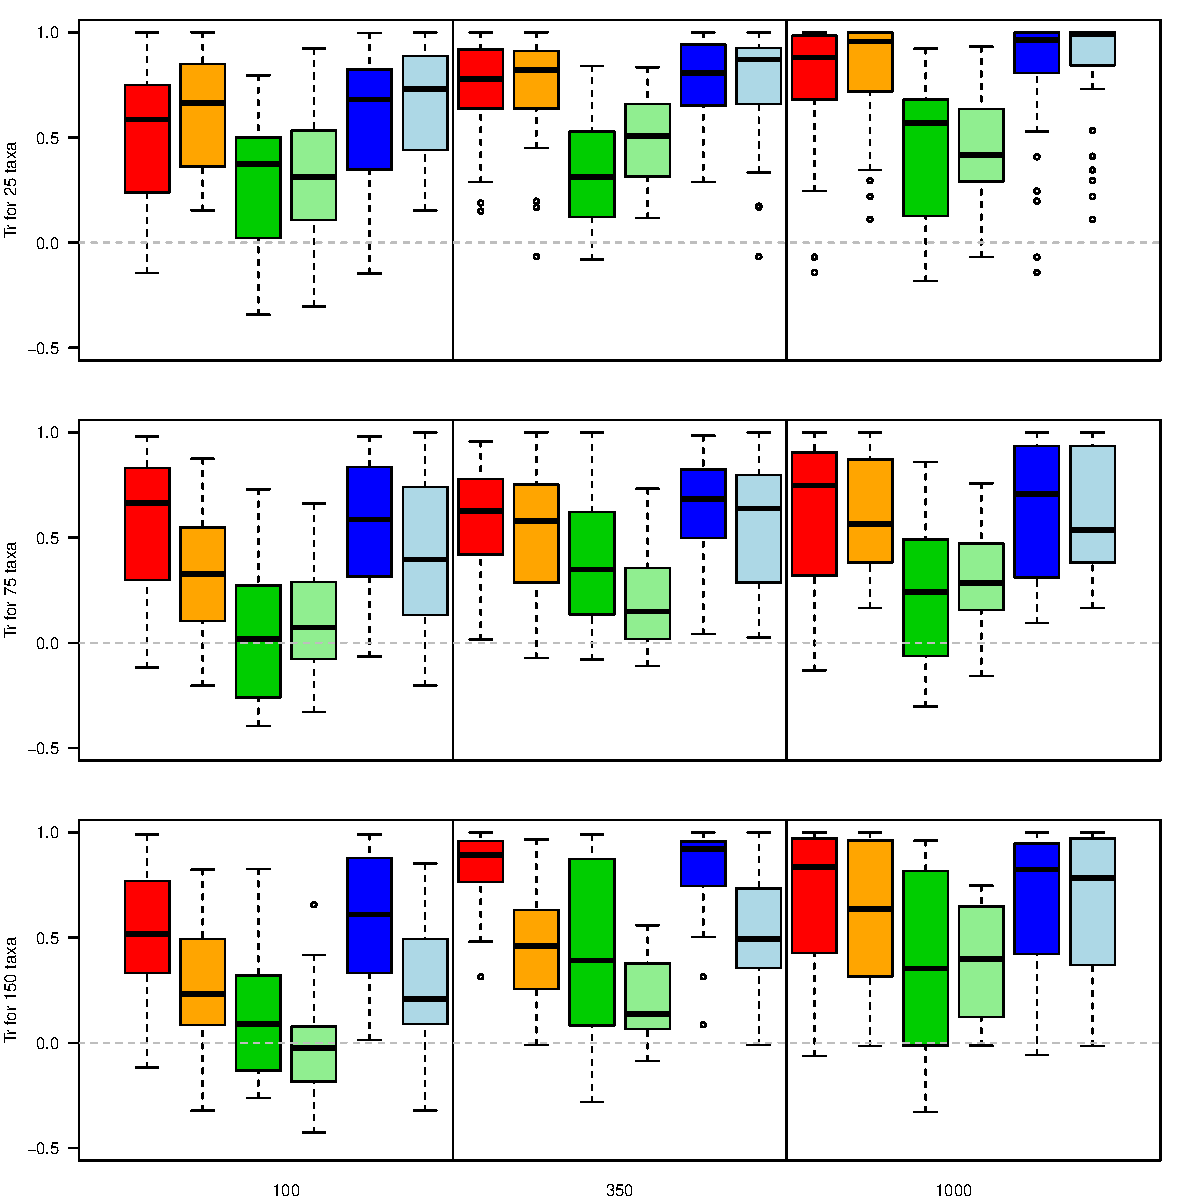
\includegraphics[width=1\textwidth]{Figures/Tr_results_null.pdf} %TG: These figures will be cleaned up once I have the final results.
\caption{Effect of Character Difference on recovering the ``random'' topology. The axis are identical to figure \ref{Fig:RF_results_best} but y axis represents the Normalised Tree Similarity using Triplets distance.}
\label{Fig:Tr_results_rand}
\end{figure}



\section{Discussion}

This goes with former results (see Parins-Fukuchi in review.)

\subsection{Effect of character differences on topology}
As expected, reducing character difference reduces the ability of recovering the best tree topology since the ``assumption'' of character independence is ``violated''.
Conversely increasing character difference increases the ability of recover the best tree topology.
However this has not more effect of topology than simply bootstrapping the matrix.

\subsection{Effect of character differences on the inference method}
Scenarios where the characters are most different to each other could favor Bayesian over Parsimony.
In fact, the only way to deal with it in parsimony analysis is to generate really homoplasic trees (since most character gives a different signal).
On the other hand probabilistic methods can better deal with this problem by increasing branch length to accommodate more changes in characters between taxa.


\subsection{Distinction between different character correlations}
%TG: this is linked to the story in the intro
Although both biological and evolutionary induce correlation is what we're interested, unless they are studied explicitly (through evo-devo hypothesis testing for example), coding and software induced correlation are the correlations we end up having to deal with.
In our study, we do not take into account biological correlation (because our characters are randomly simulated, we can not propose developmental or functional links between them), however, because they are simulated using evolutionary models based on Birth-Death trees, evolutionary induced correlation is present in our simulation (though not analysed specifically).
The coding induce correlation is simulated through our protocol of maximising/minimising the Character Difference metric from the ``normal'' matrix.
Finally, the software induced correlation is what is actually measured through these simulations.


About evolutionary induced correlation:
In practice, however, these linkages can only be inferred based on a phylogeny and will thus be dependant on the phylogenetic methods used.
For example, if a series of characters co-evol along a branch, this can be due to actual accumulation of evolutionary changes along this branch (e.g. characters linked to volancy along the Chiroptera branch) but could also be the result of inference biases (e.g. when long branch attraction occurs).


\subsection{Conclusion}
Character differences as a proxy for character correlation is not a problem \textit{per se} as long as characters are not actively coded to be similar.
On the other hand, actively selecting characters based to favor independence does not increase the ability of recovering tree topology more than bootstrapping the characters.

\section{Data availability and repeatability}
The consensus trees are available on figshare at \url{@@@}.
The code for reproducing the simulation is available and explained at \url{https://github.com/TGuillerme/CharactersCorrelation}.
The vignette for reproducing the analysis and the figure is available at \url{http://htmlpreview.github.io/?https://github.com/TGuillerme/CharactersCorrelation/Analysis/EffectCorrelation.html}.


\section{Funding}
European Research Council under the European Union’s Seventh Framework Programme (FP/2007–2013)/ERC Grant Agreement number 311092.


\section{Acknowledgements}
Calculations where done using the Imperial College London Cluster Services (doi: 10.14469/hpc/2232).
We thank Alberto Pascual Garcia for input in the design of the simulations protocol and Guillermo Herraiz Yebes for helping with the CD metric proof.


% Suggested reviewers:
%- Liliana Davalos for MPE / Joe O'Reilly, April Wright 


\bibliographystyle{sysbio}
\bibliography{References}

\end{document}

